\documentclass[12pt,a4paper]{article}
\usepackage[utf8]{inputenc}
\usepackage[spanish]{babel}
\usepackage[T1]{fontenc}
\usepackage{tocbibind} % Bibliografía en el indice
\usepackage{titlesec} % Posibilidad de editar los formatos de chapter
\usepackage{amsmath,amssymb,mathrsfs} % Matemáticas varias
\usepackage{tabularx} % Para las tablas
\usepackage[title]{appendix} % Para anexos
\usepackage[spanish]{babel} % Para modificar labels por defecto
\renewcommand{\baselinestretch}{1} % Interlineado. 1 es estandar
% --- Arreglos varios para la inclusion de imagenes
\usepackage{float}
\usepackage[pdftex]{graphicx}
\usepackage{subfigure}
\usepackage{graphicx}
\graphicspath{{T:/Tom/Facultad/Logos/}}
\usepackage[usenames,dvipsnames]{color}
\DeclareGraphicsExtensions{.png,.jpg,.pdf,.mps,.gif,.bmp}
% --- Para las dimensiones de los márgenes etc
\frenchspacing \addtolength{\hoffset}{-1.5cm}
\addtolength{\textwidth}{3cm} \addtolength{\voffset}{-2.5cm}
\addtolength{\textheight}{4cm}
% --- Para el encabezado
\setlength{\headheight}{33pt}
\usepackage{fancyhdr}
\fancyhead[R]{\includegraphics[height=1cm]{logo_fcefyn_nuevo.jpg}}\fancyhead[L]{\includegraphics[height=1cm]{unc1_a.jpg}}\fancyhead[C]{} \fancyfoot[C]{Página \thepage} \renewcommand{\footrulewidth}{0.4pt}
\pagestyle{fancy}
% --- Para las tablas
\usepackage{multirow} % Juntar filas
\newcolumntype{L}[1]{>{\raggedright\arraybackslash}p{#1}} % Justificar Izq
\newcolumntype{C}[1]{>{\centering\arraybackslash}p{#1}} % Justificar Centrar
\newcolumntype{R}[1]{>{\raggedleft\arraybackslash}p{#1}} % Justificar Der
\usepackage[numbered]{bookmark} % Para que figure las secciones en el PDF
\usepackage{listings} % Para poner código 
\usepackage{enumitem} % Para editar las propiedades de los items
\usepackage{color}
\usepackage[bottom]{footmisc} % Para las notas al pie de la página
\lstset{frame=single} % Código en un cuadro
% --- Para Anexo
\addto\captionsspanish{%
  \renewcommand\appendixname{ANEXO}
  \renewcommand\appendixpagename{ANEXOS}
}
% -------------------------------------------------------- %
% Definicion de colores para el codigo
\lstdefinelanguage{XML}
{
  basicstyle=\ttfamily\footnotesize,
  morestring=[b]",
  moredelim=[s][\bfseries\color{Maroon}]{<}{\ },
  moredelim=[s][\bfseries\color{Maroon}]{</}{>},
  moredelim=[l][\bfseries\color{Maroon}]{/>},
  moredelim=[l][\bfseries\color{Maroon}]{>},
  morecomment=[s]{<?}{?>},
  morecomment=[s]{<!--}{-->},
  commentstyle=\color{DarkOliveGreen},
  stringstyle=\color{blue},
  identifierstyle=\color{red}
}

\renewcommand{\lstlistingname}{Código}

% -------------------------------------------------------- %

\begin{document}

\begin{titlepage}
    \begin{center}
        \vspace*{1cm}
        
        \Large
        \textbf{Universidad Nacional de Córdoba\\
        		Facultad de Ciencias Exactas, Físicas y Naturales}
        
        \vspace{0.5cm}
        \includegraphics[width=0.5\textwidth]{logo_caratula.png}
        
        \vspace{1cm}
        
        \textbf{Trabajo Práctico Integrador}\\
        Programación Concurrente\\
        Docentes: \\
        Ing. Orlando Micolini\\
        Ing. Luis Ventre
        
        \vfill  
        
        \vspace{0.5cm}
        

        Alumnos:\\
        \Large
        Navarro, Sebastián\\
        
        \begin{large}
        \href{mailto:navarrosebastian95@gmail.com}{navarrosebastian95@gmail.com}\\
		\end{large} 
		
        Piñero, Tomás Santiago\\
        
        \begin{large}
        \href{mailto:tom-300@hotmail.com}{tom-300@hotmail.com}\\
		\end{large} 
		
        Año 2019\\
        
        
    \end{center}
\end{titlepage}
% -------------------------------------------------------- %
% --- Tabla de contenidos

\setcounter{secnumdepth}{1}
\setcounter{tocdepth}{5}
\tableofcontents

% -------------------------------------------------------- %

\newpage
\renewcommand{\baselinestretch}{1}
\setlength{\parskip}{0.5em}

\section{Enunciado}
\label{enunciado}

En este práctico se debe resolver el control de acceso a una playa de estacionamiento con 3 entradas (calles) diferentes. En esta playa hay 2 pisos, y en cada piso pueden estacionar 30 autos. La playa cuenta con 2 salidas diferentes y una única estación de pago (caja). En los accesos a la playa y en los egresos existen barreras que deben modelarse.

La playa cuenta con lugares (3) donde los vehículos se detienen cuando quieren entrar (barrera), una vez que ingresaron se les indica un piso y estacionan (puede ser piso 1 o piso 2). Se debe cuidar que no se permita el ingreso (superar barrera) a más vehículos de los espacios disponibles totales.

Los autos que se retiran de la playa deben liberar un espacio del piso en que se encontraban (diferenciar estacionamiento en cada piso). Cuando un vehículo se va a retirar puede optar por salida a calle 1 o salida a calle 2.
Luego debe abonar la estadía. El cobro de la estadía le lleva a un empleado promedio al menos 3 minutos. (Existe una sola caja)

En caso de que la playa esté llena, se debe encender un cartel luminoso externo que indica tal situación.

El sistema controlador debe estar conformado por distintos hilos, los cuales deben ser asignados a cada conjunto de responsabilidades afines en particular. Por ejemplo: Ingreso de vehículos, manejo de barreras, etcétera.

Debe realizar:
\begin{enumerate}
\item La red de Petri que modela el sistema.
\item Agregar las restricciones necesarias para evitar interbloqueos ni accesos cuando no hay lugar, mostrarlo con la herramienta elegida y justificarlo.
\item Simular la solución en un proyecto desarrollado con la herramienta adecuada (explique porque eligió la herramienta usada).
\item Colocar tiempo en las estación de pago caja (en la/s transición/es correspondiente/s).
\item Hacer la tabla de eventos.
\item Hacer la tabla de estados o actividades.
\item Determinar la cantidad de hilos necesarios (justificarlo)
\item Implementar dos casos de Políticas para:

\begin{itemize}
\item Prioridad llenar de vehículos planta baja (piso 1) y luego habilitar el piso superior. Prioridad salida indistinta (caja).
\item Prioridad llenado indistinta. Prioridad salida a calle 2.
\end{itemize}

\item Hacer el diagrama de clases.
\item Hacer los diagramas de secuencias.
\item Hacer el código.
\item Hacer el testing.
\end{enumerate}

\section{Desarrollo}
\label{desarrollo}

\subsection{Tabla de estados.}
\begin{table}[H]
\centering
\begin{tabular}[width=15cm]{ || C{1.5cm} | L{5cm} | L{8.5cm} || }
\hline
	Numero & Plaza & Estado  \\ \hline
	P0 & Limitador clientes calle 1 & Buffer que limita la cantidad de clientes a ingresar por la primer calle  \\ \hline
	P1 & Limitador clientes calle 2 & Buffer que limita la cantidad de clientes a ingresar por la segunda calle \\ \hline
	P2 & Limitador clientes calle 3 & Buffer que limita la cantidad de clientes a ingresar por la tercer calle  \\ \hline
	P3 & Autos esperando ingresar calle 1 & Cola de autos esperando para sacar el ticket en la primer calle  \\ \hline
	P4 & Autos esperando ingresar calle 2 & Cola de autos esperando para sacar el ticket en la segunda calle\\ \hline
	P5 & Autos esperando ingresar calle 3 & Cola de autos esperando para sacar el ticket en la tercer calle \\ \hline
	P6 & Auto pasando barrera 1 & El cliente sacó el ticket y la barrera se levanta  \\ \hline
	P7 & Auto pasando barrera 2 & El cliente sacó el ticket y la barrera se levanta   \\ \hline
	P8 & Auto pasando barrera 3 & El cliente sacó el ticket y la barrera se levanta  \\ \hline
	P9 & Barrera de calle 1 & Mutex para el uso de la barrera de la primer calle   \\ \hline
	P10 & Barrera de calle 2 & Mutex para el uso de la barrera de la segunda calle  \\ \hline
	P11 & Barrera de calle 3 & Mutex para el uso de la barrera de la tercer calle  \\ \hline
	P12 & Limitador de autos & Buffer que limita la cantidad de autos a utilizar la rampa  \\ \hline
	P13 & Autos por tomar rampa & Autos utilizando la rampa \\ \hline
	P14 & Auto buscando lugar arriba & Cliente buscando lugar para estacionar el auto en planta alta \\ \hline
	P15 & Auto buscando lugar abajo & Cliente buscando lugar para estacionar el auto en subsuelo \\ \hline
	P16 & Rampa & Mutex de uso de la rampa  \\ \hline
	P17 & Auto estacionado arriba & Auto estacionado en la planta de arriba  \\ \hline
	P18 & Auto estacionado abajo & Auto estacionado en el subsuelo  \\ \hline
	P19 & Lugares disponibles arriba & Cantidad de lugares disponibles en la planta alta \\ \hline
	P20 & Lugares disponibles abajo & Cantidad de lugares disponibles en el subsuelo  \\ \hline
	P21 & Cliente pagando arriba & Cliente sale de la planta alta y abona el ticket   \\ \hline
	P22 & Cliente pagando abajo & Cliente sale del subsuelo y abona el ticket  \\ \hline
	P23 & Auto en rampa & Cliente esta bajando o subiendo por la rampa  \\ \hline
	P24 & Cliente por pagar & Cliente esperando para pagar el ticket  \\ \hline
	P25 & Cliente pagando & Cliente pagando el ticket \\ \hline
\end{tabular}
\end{table}
\begin{table}[H]
\centering
\begin{tabular}[width=15cm]{ || C{1.5cm} | L{5cm} | L{8.5cm} || }
\hline
	P26 & Cajero & Cajero \\ \hline
	P27 & Auto por salir & Auto por abandonar la playa de estacionamiento \\ \hline
	P28 & Limitador de playa & Buffer que limita la cantidad de clientes que pueden ingresar al estacionamiento \\ \hline
\end{tabular}
\caption{Tabla de estados.}
\label{table:plazas}
\end{table}

\subsection{Tabla de eventos.}
\begin{table}[H]
\centering
\begin{tabular}[width=15cm]{ || C{1.5cm} | L{5cm} | L{8.5cm} || }
\hline
	Numero & Plaza & Estado  \\ \hline
	T0 & Entrar calle 1 & Autos ingresando por la primer calle  \\ \hline
	T1 & Entrar calle 2 & Autos ingresando por la segunda calle \\ \hline
	T2 & Entrar calle 3 & Autos ingresando por la tercer calle \\ \hline
	T3 & Sacar ticket 1 & El cliente saca el ticket para levantar la barrera  \\ \hline
	v4 & Sacar ticket 2 & El cliente saca el ticket para levantar la barrera \\ \hline
	T5 & Sacar ticket 3 3 & El cliente saca el ticket para levantar la barrera \\ \hline
	T6 & Levantar barrera 1 & Una vez sacado el ticket, se levanta la barrera para el ingreso a la playa  \\ \hline
	T7 & Levantar barrera 2 & Una vez sacado el ticket, se levanta la barrera para el ingreso a la playa   \\ \hline
	T8 & Levantar barrera 3 & Una vez sacado el ticket, se levanta la barrera para el ingreso a la playa  \\ \hline
	T9 & Subir por rampa & El cliente sube a la planta alta del estacionamiento   \\ \hline
	T10 & Bajar por rampa & El cliente va a la planta baja del estacionamiento  \\ \hline
	T11 & Buscar lugar arriba & El cliente busca lugar para estacionar en la planta alta  \\ \hline
	T12 & Buscar lugar abajo & El cliente busca lugar para estacionar en la planta baja  \\ \hline
	T13 & Aguardar salida arriba & El cliente dejó el auto estacionado en la planta alta \\ \hline
	T14 & Aguardar salida abajo & El cliente dejó el auto estacionado en la planta baja \\ \hline
	T15 & Bajar & El cliente de la planta alta se dirige a la salida \\ \hline
	T16 & Subir & El cliente de la planta baja se dirige a la salida  \\ \hline
	T17 & Esperar caja & El cliente se dirige a la caja  \\ \hline
	T18 & Pagar & El cliente paga el ticket en la caja  \\ \hline
	T19 & Devolver cajero & El cliente elige la salida \\ \hline
	T20 & Salir por calle 1 & El cliente sale por la calle 1  \\ \hline
	T21 & Salir por calle 2 & El cliente sale por la calle 2   \\ \hline
\end{tabular}
\caption{Tabla de eventos.}
\label{table:plazas}
\end{table}

\subsection{Hilos}
 Los hilos son aquellos que realizan un conjunto de acciones, por lo que para determinar la cantidad de hilos necesarios, se realizó una modularización de la red en actividades, por lo tanto, la cantidad de hilos utilizados son 8

\begin{enumerate}[leftmargin=1.5cm]
\item Entrada calle 1: T0 - T3.
\item Entrada calle 2: T1 - T4.
\item Entrada calle 3: T2 - T5.
\item Asignar piso: T6 - T7 - T8 - T9 - T10.
\item Planta Alta: T11 - T13 - T15.
\item Planta Baja: T12 - T14 - T16.
\item Cobrar tickets: T17 - T18 - T19.
\item Salida: T20 - T21.
\end{enumerate}
\subsubsection*{Hilos 1, 2 y 3.}
Los 3 hilos iniciales en las entradas son de existencia trivial, donde cada calle (o entrada) es independiente una de la otra, y cada una cuenta con sus propios recursos. La red resultante en este bloque será el estado inicial para el hilo 4.
\subsubsection*{Hilo 4.}
La segunda etapa de la red, el tramo que abarca el acceso y la asignación de piso, arriba o abajo, es ejecutada mediante un solo hilo.
Este hilo resulta indispensable para la fluidez de la red. Al ser el conjunto de transiciones con más actividad, resulta necesario contar con un hilo que siempre tenga alguna de sus transiciones sensibilizadas, de modo que éste se encole la menor cantidad de veces posible y en consecuencia, los alrededores de la red no conduzcan a un interbloqueo.
Además, al asignarle las transiciones T9 y T10 que introducen conflicto, facilita la implementación de políticas para resolverlo.
\subsubsection*{Hilos 5, 6 y 7.}
Se independizan esos 3 conjuntos de transiciones de la red para modularizar lo más posible y así elevar la concurrencia de la red.
\subsubsection*{Hilo 8.}
Se asigna un hilo a la dupla de transiciones T20 y T21 para resolver el último conflicto de la red, de modo que se puede implementar más fácilmente una política que las administre, y que además asegure un comportamiento consistente. 

\subsection{Red de Petri.}
\begin{figure}[H]
    \centering
    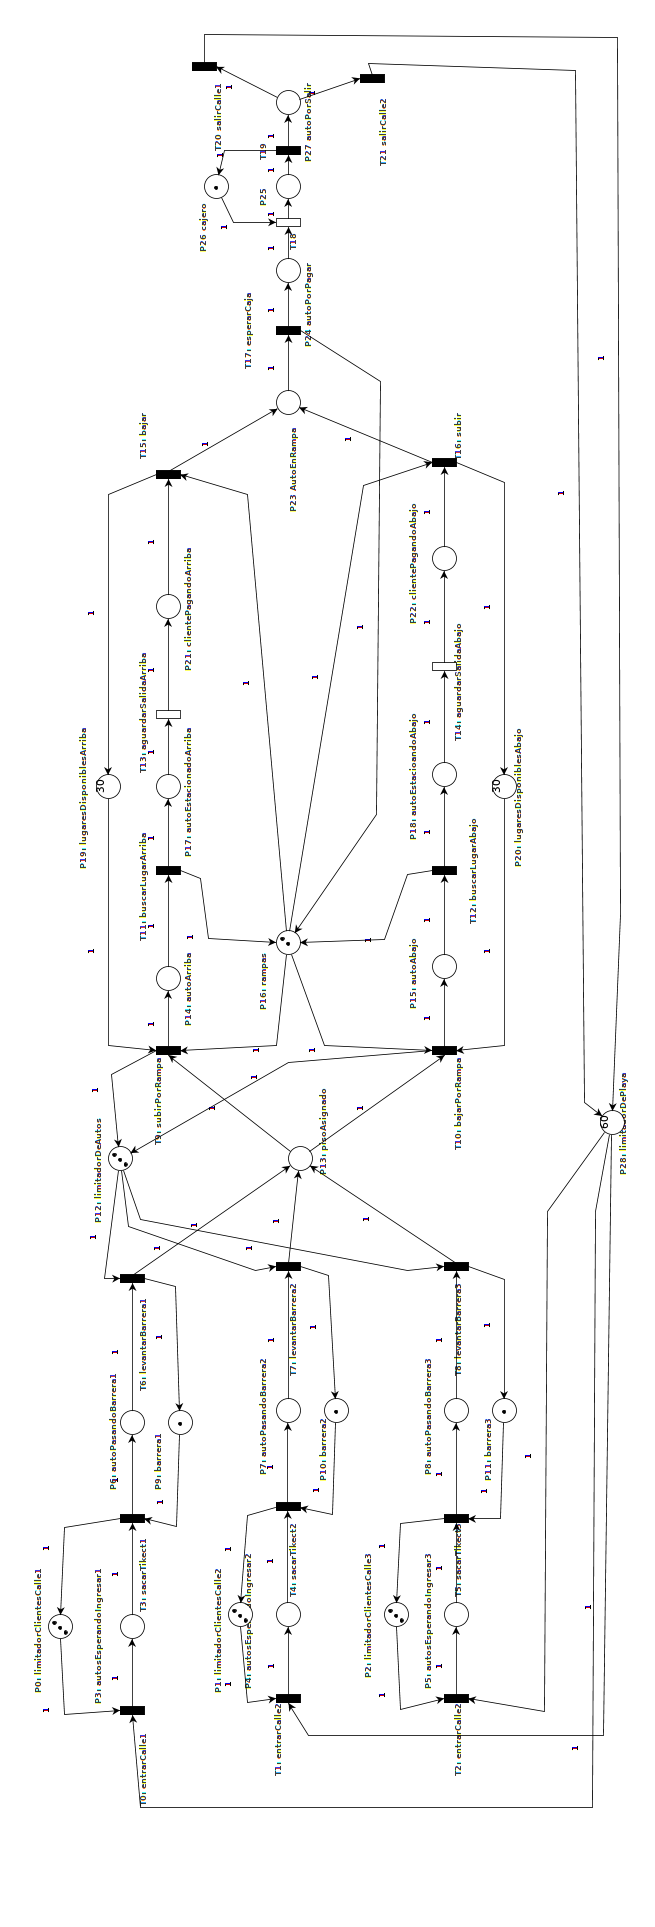
\includegraphics[scale=0.34]{./estacionamiento_2019}
    \label{fig:rdp}
\end{figure}{}

Haremos uso de una clase dedicada a cronometrar aquellas transiciones temporizadas. 

Una transición con tiempo se cronometra desde el inicio de la sensibilización de la transición, y en el momento en el que se quiere disparar, se debe verificar que el tiempo dicho esté dentro del intervalo de tiempo $[a_i , b_i]$.

Si el disparo se quiere realizar antes del límite inferior $(a_i)$, el hilo debe dormir $a_i-x$ segundos, donde $x$ es el tiempo transcurrido desde que se sensibilizó la transición.

\textbf{Semántica utilizada para las transiciones temporizadas.}

Se tomo la primera de las semánticas especificadas en \textit{“Redes\textunderscore de\textunderscore  Petri\textunderscore Temporales\textunderscore 2017.pdf” - Hoja 11}, por lo tanto el disparo se realiza en dos etapas:
\begin{itemize}
    \item Transcurre un determinado tiempo desde que una transición se sensibiliza
    \item Se retiran y colocan las marcas de forma atómica
\end{itemize}
Cabe mencionar que esto se usa para ambos tipos de transiciones: inmediatas y temporales, ya que en el caso de la inmediata, el paso 1 implica un intervalo de tiempo nulo.

\subsection{Políticas}
Aquel conjunto de transiciones pertenecientes a un hilo en particular, que no requieran el tratado de políticas específicas, se dispararán de forma consecutiva siguiendo una secuencia de bucle para garantizar el orden y la fluidez de la red.

En el caso en que la prioridad de la transición sea indistinta, se elegirá la primera de las transiciones que corresponden al hilo segun el orden que llevan en el archivo ‘hilos.txt’, de modo que este orden puede suponerse como un orden de prioridades.

Por otro lado, las transiciones que requieren tratado de politicas especificas, son administradas por la clase Politicas del proyecto y obedecen al enunciado.



\end{document}